\section{Performance}
\label{sec:performace}

We've evaluated Tutamen in a variety of scenarios using the
applications described in \S~\ref{sec:apps}. These scenarios have
proven Tutamen's usefulness as an enabler of previously unattainable
functionally and use cases. While Tutamen is still a prototype, we
feel it provides a well designed architecture capable of supporting a
wide range of practical secret storage applications. While the server
software has not yet been optimized for performance, we have performed
a number of performance measurements in order to better understand the
relative computational load and bottlenecks of the various parts of
the Tutamen system.

\begin{figure}[th]
  \centering
  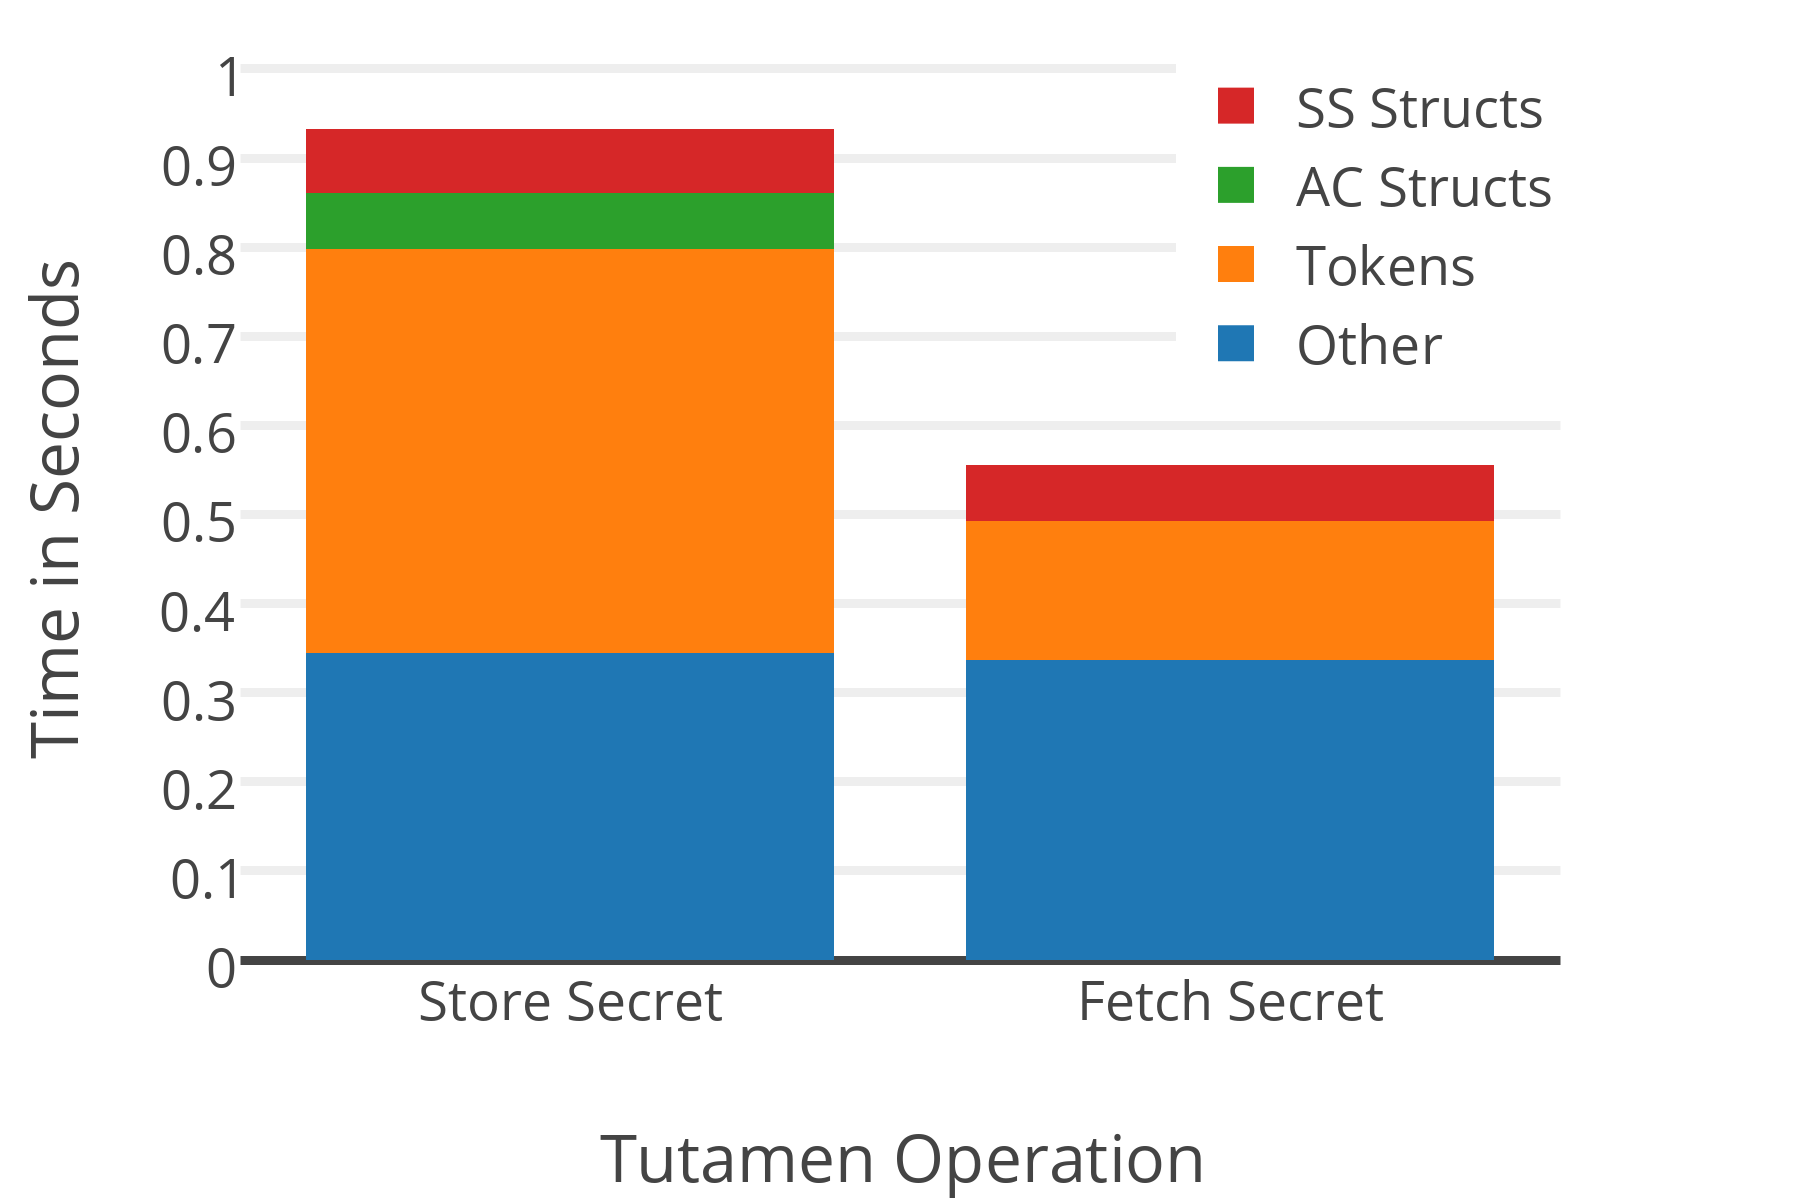
\includegraphics[width=\columnwidth]{./figs/png/chart-timings.png}
  \caption{Timings for Tutamen Operations}
  \label{fig:eval:timings}
\end{figure}

Figure~\ref{fig:eval:timings} shows the time required to complete two
of the most common Tutamen operations: storing a new secret and
retrieving a previously stored secret. We profiled the amount of time
the Tutamen CLI application spent performing various parts of each of
these two Tutamen operations. In both operations, the bulk of the
wait-on-server-related run time is spent requesting and retrieving the
authorization tokens required to complete the associated
operations. In the secret creation case, five tokens are
required\footnote{Two permissions group creation tokens (one for the
  collection permission group and one for the verifier itself), one
  verifier creation token, one collection creation token, and one
  secret creation token.}. In the secret read case only a single token
is required\footnote{The collection read permission token}. The
remainder of the server-related time is spent either creating AC and
storage data structures (as in the store secret case) or reading
existing data structures (as in the retrieve secret case). The
``other'' time is spent reading the Tutamen config files, loading the
necessary client certificates, and dealing with the overhead required
to interpret the python-based CLI.

It is not unexpected that the client must spend the bulk of its time
requesting tokens and waiting for them to be approved -- token
verification is the primary role the access control server must
perform, and depending on the complexity of the verifiers associated
with the permission the token is requesting, verification can be a
fairly complex task. When performing these measurements, we employed a
simple verifier that only required client membership in a specific
account. Verifiers that include human-in-the-loop authenticators
(e.g. SMS approval) would increase the token turnaround time by the
amount of time the human requires to provide approval. Thus, it's
important that Tutamen applications treat token approval as an
operation that can take anywhere from under a second to human-scale
times (e.g. 10s of seconds). To help alleviate these waits on
applications that must perform a high number of Tutamen requests,
Tutamen tokens may be reused up until their expiration time. Thus, its
possible for an applications to request a long lived token and to
reuse this token to access multiple secrets within the collection to
which the token grants read access.
 
\begin{figure}[th]
  \centering
  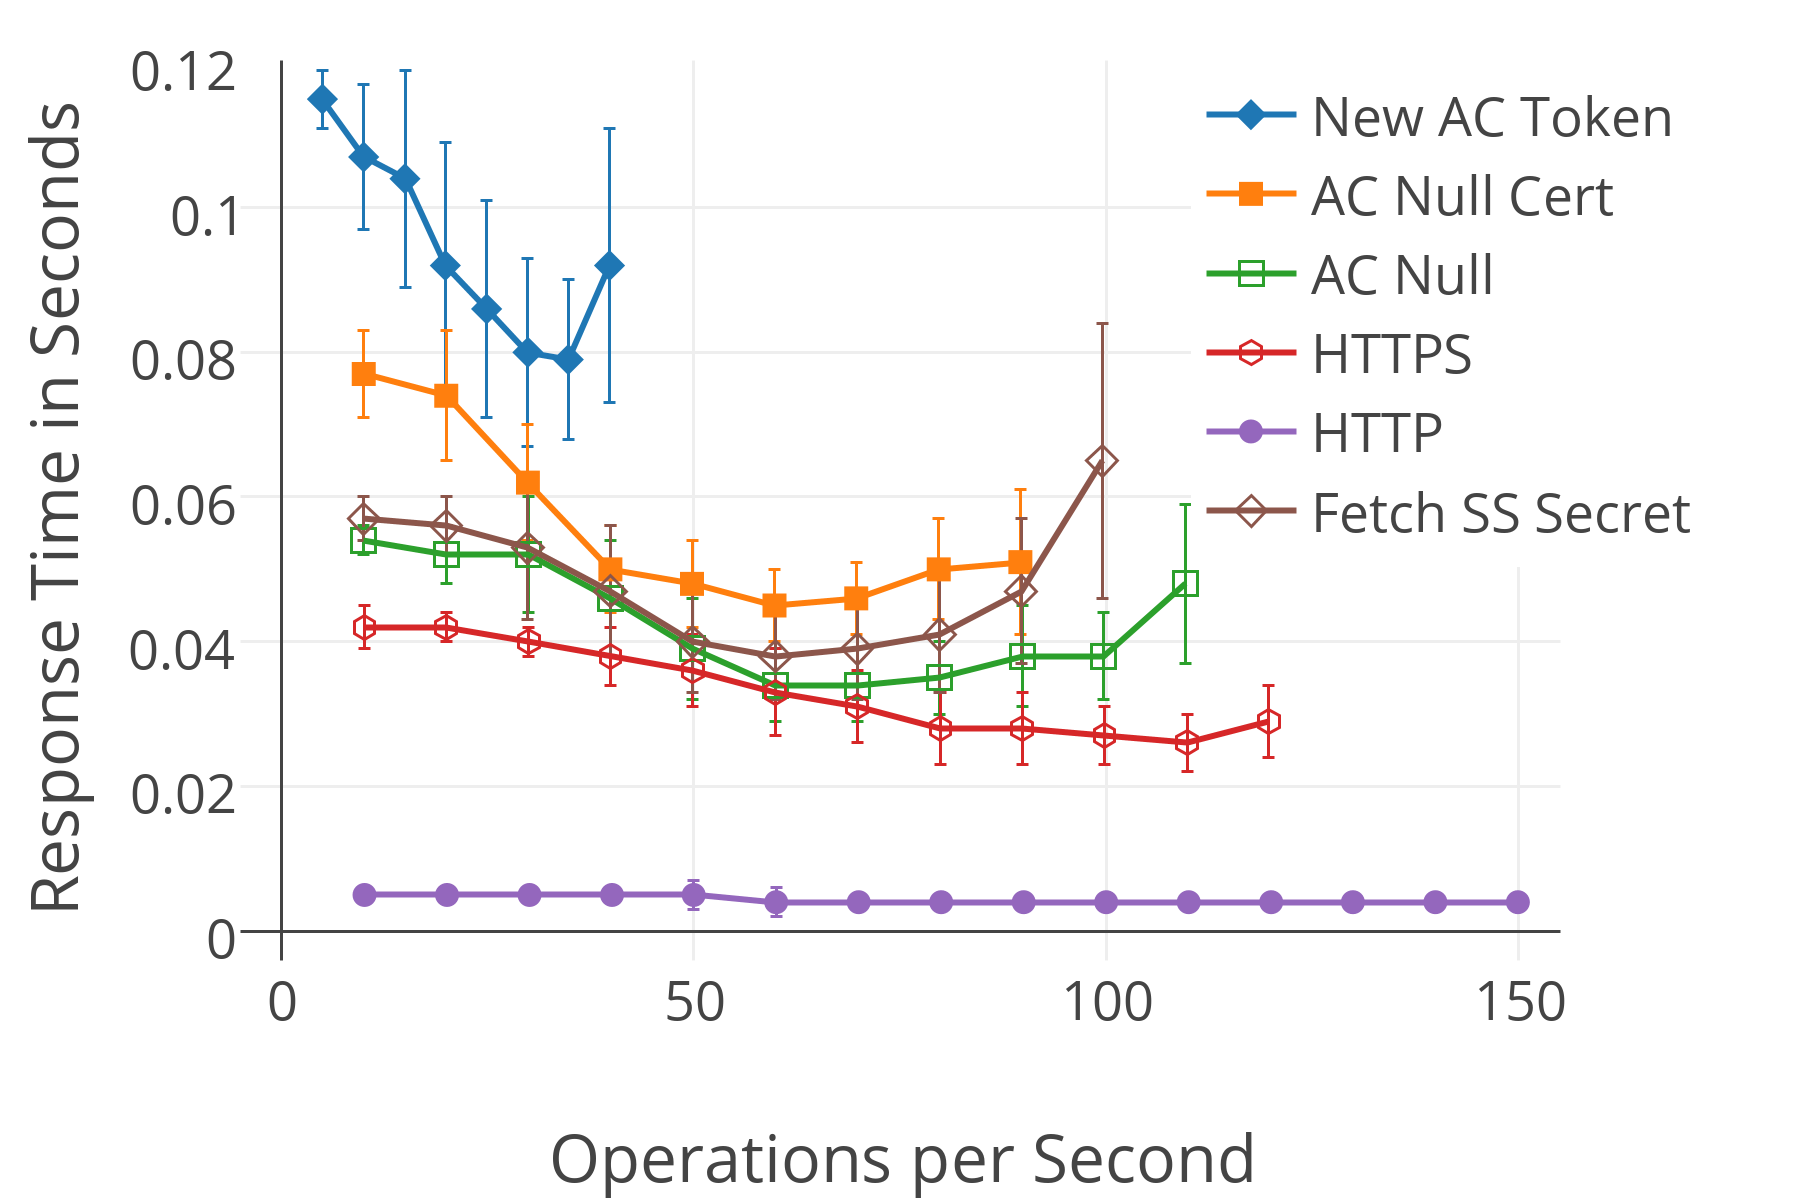
\includegraphics[width=\columnwidth]{./figs/png/chart-iops.png}
  \caption{Throughput vs Latency Curves}
  \label{fig:eval:iops}
\end{figure}

Figure~\ref{fig:eval:iops} shows the request rate vs response time
(with standard deviations) of a token request operation, two ``null''
AC API operations (one that sends and verifies the client TLS
certificate and one that does not) and a fetch secret operation. Raw
Apache HTTPS and HTTP curves are also shown for comparison. As these
curves show, token verification of our prototype server tops out at
around 40 requests/second (rps) on a modest server (2-core, 4GB VM
running atop 2011-era Intel Xeon hardware). The null AC API operation
with client certificates tops out around 90 rps and the null operation
without client certificates tops out at about 110 rps. Raw HTTPS tops
out around 120 rps. HTTP topped out around 5000 rps (curve truncated
for view-ability). The current server setup is thus primarily limited
by the crypto overhead required to serve the application and verify
client certificates using TLS. Token verification itself also incurs
additional computational requirements, but is well within the order of
magnitude of the underlying server limits themselves. Secret retrieval
(after acquiring a token) is relatively quick topping out around 100
rps.

While these levels of performance would not likely meet the
requirements of a production-level Tutamen AC server, they have been
perfectly adequate for our needs supporting the handful of Tutamen
applications we're currently using and experimenting with. Since most
of our Tutamen applications require only a single Tutamen secret
retrieval at relatively rare rates (e.g. once per server reboot, or
once per file open) the 40+ requests per second our AC server can
provide have been more than adequate for our needs. We've also
designed our reference server to be horizontally scalable in both its
HTTPS request handling (e.g. by spinning up multiple load-balanced API
servers. That scalability, coupled with future performance-related
code optimization, lead us to believe the Tutamen server
infrastructure can be adopted to meet the needs of larger
installations with only moderate effort. It's also likely that
enabling additional crypto-acceleration options (such as Intel's
AES-NI) would help reduce the TLS overhead imposed on each Tutamen
server.

%%  LocalWords:  Tutamen Tutamen's verifiers authenticators SMS Xeon
%%  LocalWords:  authenticator HTTPS Redis
